\documentclass[12pt]{article} % ein Artikel in 11-Punkt Schrift
% wie man sich schon denkt leitet % einen Kommentar bis Zeilenende ein

\usepackage[german]{babel} % deutsch, deutsche Rechtschreibung
\usepackage[utf8]{inputenc} % Unicode Text 
\usepackage[T1]{fontenc} % Umlaute und deutsches trennen
\usepackage{mathptmx} % Times New Roman, gewohnter Font
\usepackage{courier} % Schreibmaschinenfont schicker
\usepackage[scaled=.95]{helvet} % was serifenloses wenn gebraucht
\usepackage{graphicx} % wir wollen Bilder einfügen

\usepackage{listings} % Schöne Quellcode-Listings
\lstset{basicstyle=\sffamily, columns=[l]flexible, mathescape=true, 
  showstringspaces=false, numbers=left, numberstyle=\tiny}
\lstset{language=python} % und nur schöne Programmiersprachen ;-)
% und eine eigene Umgebung für Listings
\usepackage{float}
\newfloat{listing}{htbp}{scl}[section]
\floatname{listing}{Listing}

% Auch wenn es anrüchig ist, man kann den Platz etwas mehr ausnützen
\usepackage[paper=a4paper,width=14cm,left=35mm,height=22cm]{geometry}
\usepackage{setspace}
\linespread{1.25} % nicht ganz anderthalbzeilig, nur ein bisschen mehr Platz
\setlength{\parskip}{0.5em} % kleiner Paragraphenabstand
\setlength{\parindent}{0em} % im Deutschen Einrückung nicht üblich, leider

% Seitenmarkierungen 
\usepackage{fancyhdr} % Schickere Header und Footer
\pagestyle{fancy}
% Zeichensatz für Header/Footer
\newcommand{\phv}{\fontfamily{phv}\fontseries{m}\fontsize{9}{11}\selectfont}
\fancyhead[L]{\phv Praktikumsbericht} 
\fancyhead[R]{\phv \thepage}
\fancyfoot[L]{\phv Hochschule RheinMain}
\fancyfoot[C]{\ } % keine Seitenzahl unten
\fancyfoot[R]{\phv Medieninformatik}

% Ein spezielles Paket zum Aufteilen des Literaturverzeichnisses
% \usepackage{bibtopic}
\usepackage{url} % wir wollen eine URL anzeigen

\title{Exposé für eine Bachelorarbeit zum Thema:\newline Interaktive 3D Echtzeitvisualisierung von Luftreinheitsdaten}
\author{Joshua Coelho Mestre}
\date{\today} % oder \today für heute

\begin{document}

\maketitle
% \begin{abstract}
  % Exposé für eine Bachelorarbeit zum Thema: 3D Echtzeit Datenvisualisierung von Luftreinheitsdaten.
% \end{abstract}
\newpage
\tableofcontents % das Inhaltsverzeichnis
\newpage % neue Seite, muss bei einem Artikel eigentlich nicht sein

\section{Problemstellung} \label{sec:Problemstellung}

Wir leben in einer Zeit in der unteranderem durch Skandale wie die Diesel"=Abgasaffäre das Thema Luftreinheit in unseren Städten in den Fokus der öffentlichen Aufmerksamkeit gerückt ist.
Obwohl das Thema in den letzten Jahren so präsent wie nie zuvor ist scheint es noch einige Menschen zu geben denen der Ernst der Lage noch nicht bewusst ist.

Sowohl die Feinstaub"= als auch die Stickoxid (NOx)-Belastungen in deutschen Innenstädten reizen vielerorts die gesetzlichen und gesundheitlich zumutbaren Grenzewerte aus. Und das obwohl bekannt ist, dass eine hohe Feinstau-Belastung erhebliche gesundheitliche Risiken mit sich bringt.

Die winzigen Partikel können ab einer kritischen Größe über die Atemwege direkt in die menschliche Blutbahn eindringen, was zu Folge hat, dass Menschen, die in besonders belasteten Regionen leben ein höheres Risiko haben an Schlaganfällen, Herzleiden und Atemwegserkrankungen zu erleiden.

Stickoxide reizen analog zu Feinstaub die Atemwege beim und lösen dadurch Entzündungen in Atemwegen und Lunge aus, wodurch vor allem Menschen betroffen sind die bereits an einer Lungen- oder Atemwegserkrankung leiden, da ihre Lungenfunktion zusätzlich eingeschränkt wird\cite{zo:StickoxideUndFeinstaub}.

\section{Forschungsstand} \label{sec:Forschungsstand}

Zur Zeit gibt es bereits Visualisierungen von Stickstoff-Belastung in manchen Städten. 
Allerdings wird bei den zur Zeit existierenden Visualisierungen oft nicht die gesamtdeutsche Situation beleuchtet.
Und selbst wenn dies der Fall ist beschränken sich die Visualisierungen auf die reine Darstellung der Messdaten und nur oberflächlich, wenn überhaupt, damit bei dem Betrachter eine Stimmung zu erzeugen, die zum Nachdenken anregt.

\section{Zielsetzung und Erkenntnisinteresse} \label{sec:Zielsetzung}

Ziel dieser Bachelorarbeit soll es sein dem Thema der Luftverschmutzung mehr Aufmerksamkeit zu verschaffen, indem sie die aktuellen Daten unter Berücksichtigung des gesundheitlich vertretbaren Grenzwerte visualisiert.

Die Visualisierung soll, als Installation ausgestellt werden können und in dieser Rolle ein Bewusstsein für die aktuelle Lage der Situation in deutschen Städten schaffen.
Sie soll dem Betrachter die aktuelle Lage verdeutlichen und ihn im Falle bedenklicher Messwerte dazu bewegen über eine mögliche Eigeninitiative nachzudenken.

Das konkrete Ziel ist es sowohl die Stickoxid"= als auch den Feinstaub"=Konzentration in eine optische Relation zu ihrer Schädlichkeit zu setzen. 
Je schädlicher die gemessene Konzentrationen der Schadstoffe sind desto bedrohlicher soll die Visualisierung der Messdaten sich darstellen.

Zusätzlich zu dem stimmungserzeugenden Charakter der Visualisierung soll interessierten Nutzern über eine Interaktion mit der Visualisierung die Möglichkeit gegeben werden, Auskunft über die genauen Messwerte und gegebenenfalls über die negativen gesundheitlichen Folgen dieses Wertes geben.

\section{Forschungskonzept} \label{sec:Forschungskonzept}
Im Rahmen dieser Bachelorarbeit sollen alle verfügbaren Messstationen in Deutschland durch jeweils eine Kugel repräsentiert werden.

Die Farbe und Transparenz der Kugeln richten sich nach den, an der jeweiligen Messstation gemessenen Daten.
Um den stimmungsgenerierenden Effekt der Visualisierung zu erhalten, wird für einen positiven Messwert, der sich weit unterhalb des Grenzwertes befindet, eine helle beruhigende Farbe und eine hohe Transparenz gewählt.

Je näher der gemessene Wert dem Grenzwert kommt, desto mehr soll sich die Farbe in eine dunkle und bedrohliche Farbe verändern. Gleichzeitig und analog zur Farbänderung, soll die Transparenz der Kugel abnehmen, je mehr sich die Messdaten dem Grenzwert nähern.

Bei einer deutlichen Überschreitung des Grenzwertes, soll sich die Kugel komplett schwarz färben und ihre Transparenz gänzlich verlieren, was dazu beiträgt, die Stimmung der Visualisierung bedrohlich wirken zu lassen.

Da die Visualisierung nicht sofort als eine solche erkannt werden soll, wird eine zunächst chaotische Bewegung der Kugeln erzeugt.
Mittels eines Ultraschall-Sensors wird ermittelt, ob ein Nutzer physisch vor der Visualisierung steht und diese betrachtet.

\begin{figure}
	\centering
	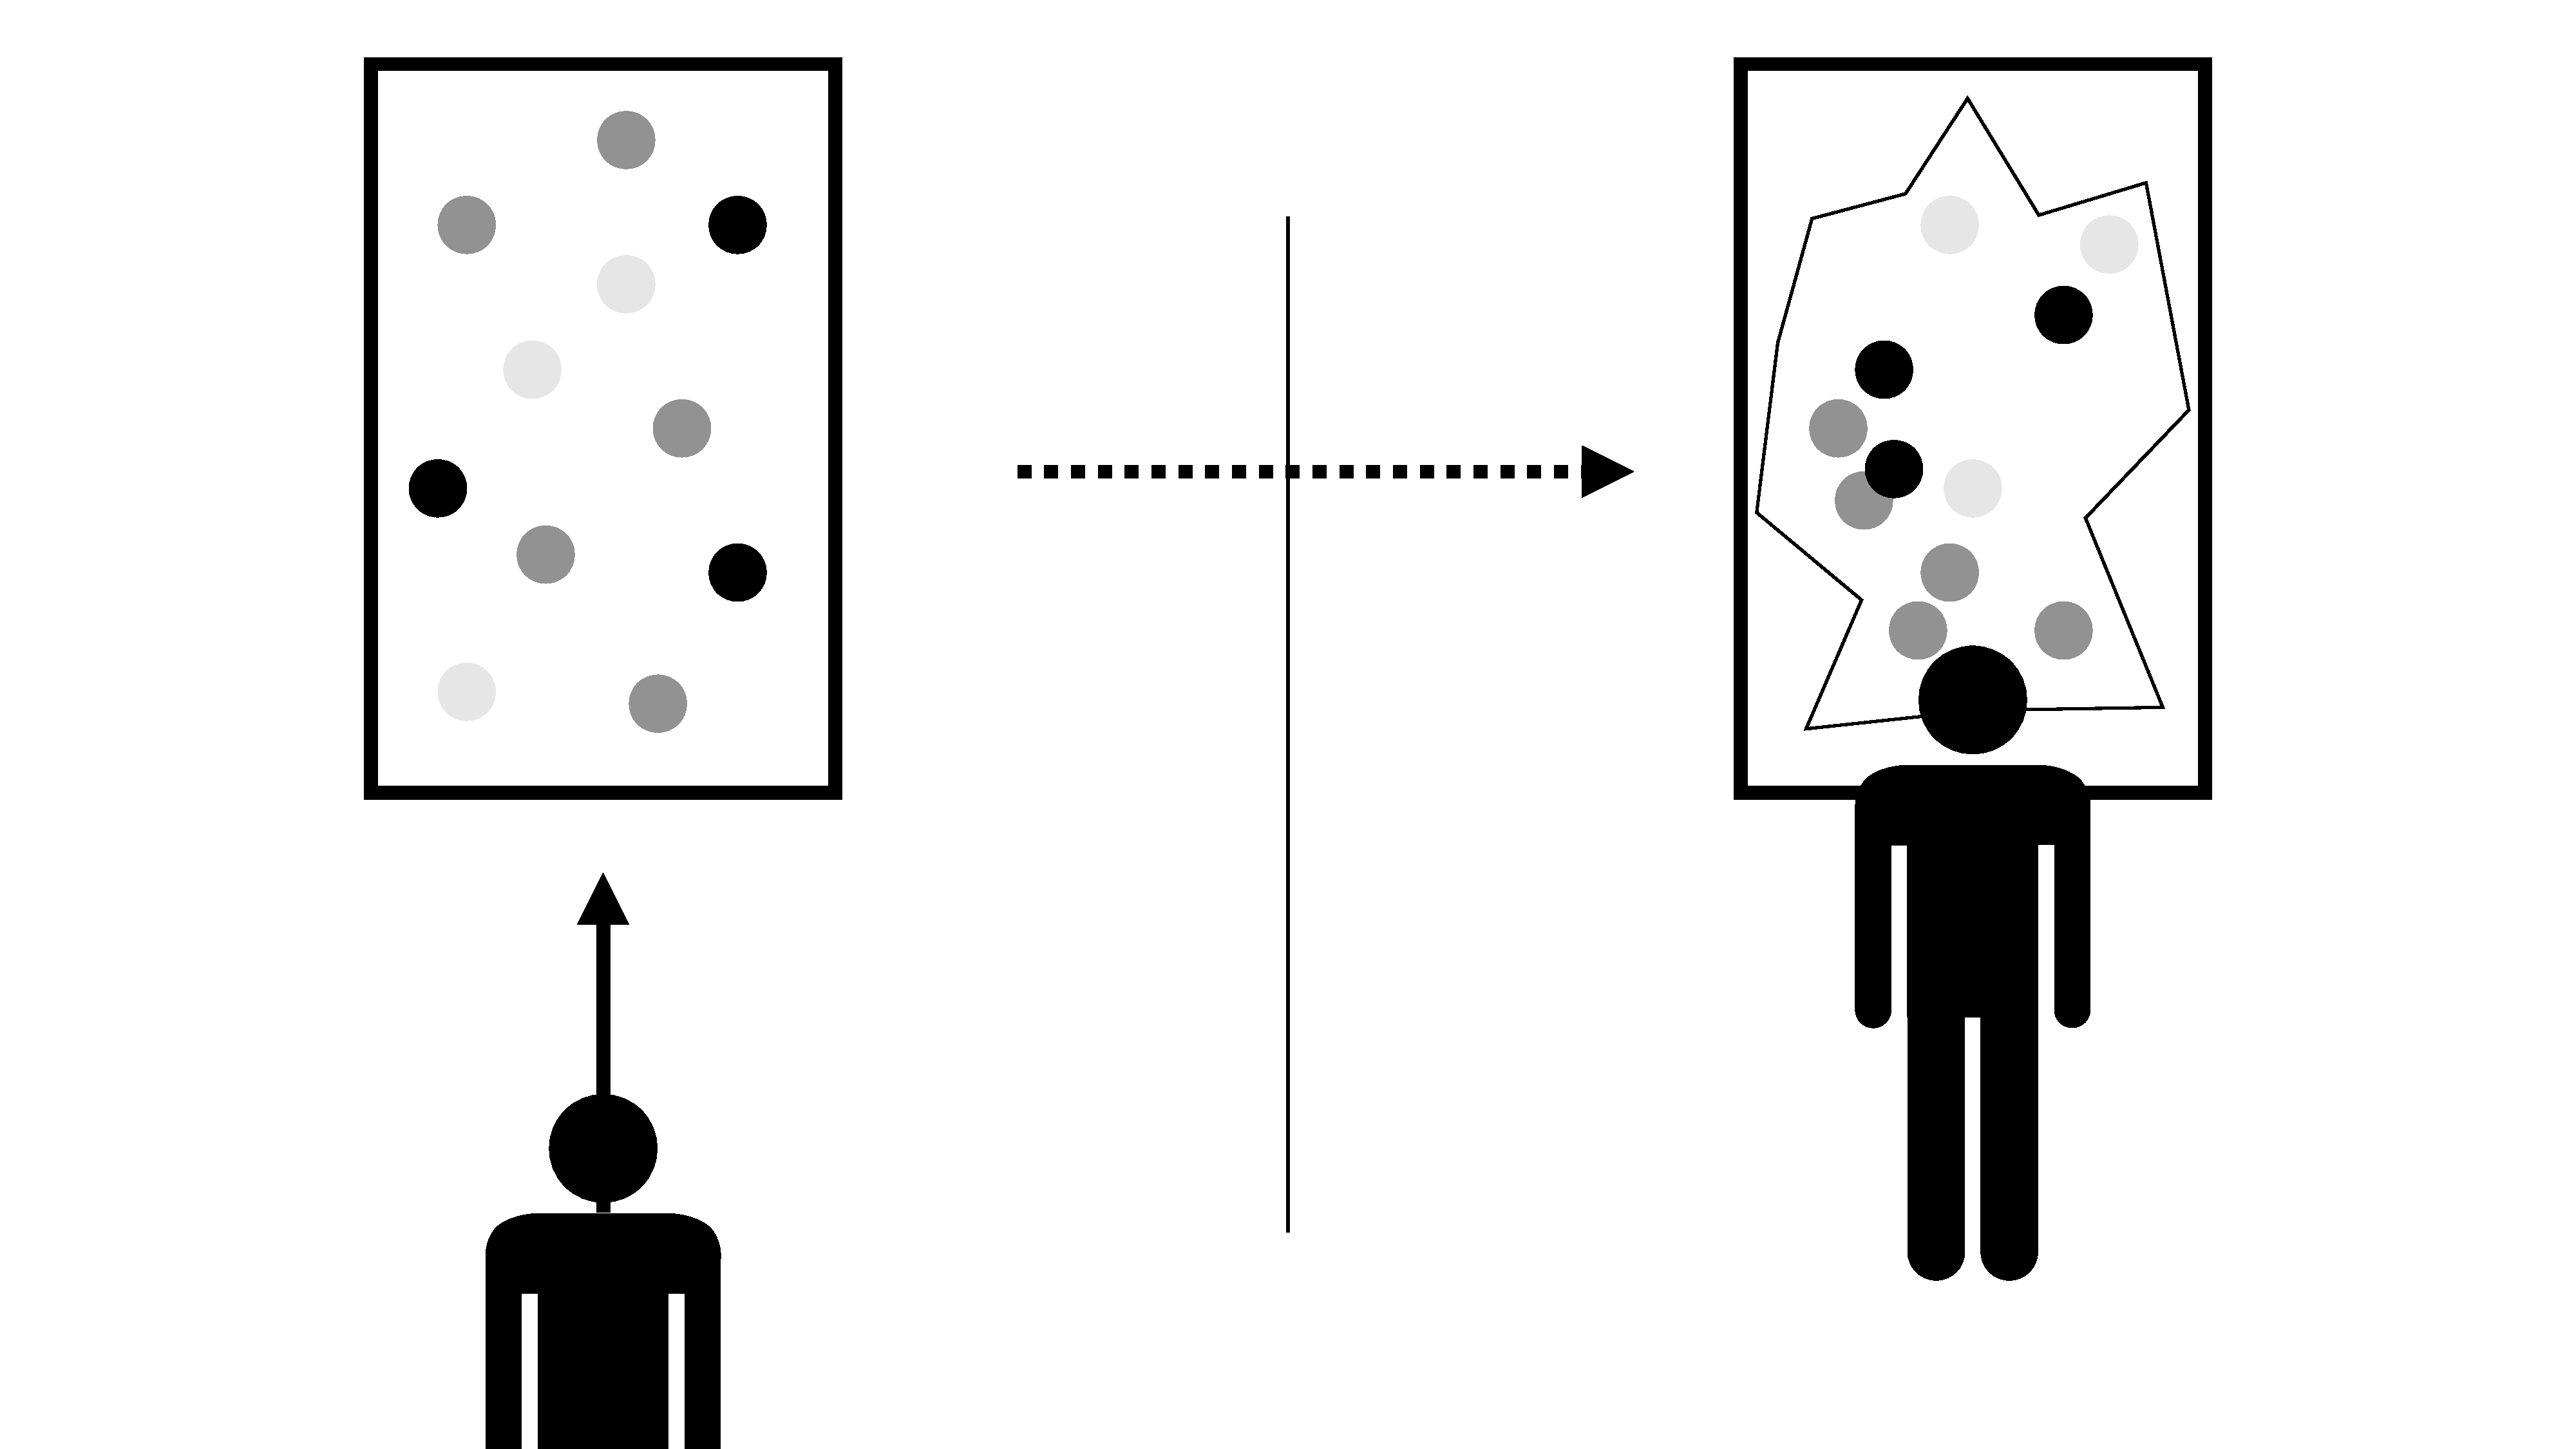
\includegraphics[scale=0.1]{assets/Diagram.pdf}
  \caption{Schematische Darstellung des Konzepts}
	\label{pdf:diagram}
\end{figure}

In diesem Fall sollen sich die Kugeln entsprechend der geografischen Lage der jeweiligen Messstation anordnen, wie in Abbildung \ref{pdf:diagram} zu sehen.
Dem Nutzer soll es daraufhin ermöglicht werden, durch einen Klick auf eine der Kugel, die Messdaten der zugehörigen Messstation einzusehen.

Nachdem sich der Nutzer wieder physisch von der Visualisierung entfernt hat, sollen die Kugeln bis zur nächsten Interaktion wieder in den chaotischen Bewegungszustand gehen.  

Das Konzept soll mithilfe eines Raspberry Pi, der sich hinter einem Bildschirm befindet, realisiert werden.
Zusätzlich soll dieser mit dem oben erwähnten Ultraschall-Abstands-Sensor ausgestattet sein. 


\section{Schwerpunkte und Herausforderungen} \label{sec:Schwerpunkte}

Der Schwerpunkt der Arbeit soll darin liegen, eine Ästhetik zu generieren, die eine von der Schadstoffbelastung abhängige Stimmung erzeugt.
Gleichzeitig soll die Visualisierung dem Nutzer die konkreten und objektiven Messdaten präsentieren.  

Die Schwierigkeit in diesem Vorhaben wird vermutlich darin liegen, die Subjektivität der stimmungserzeugenden Ästhetik mit der nüchternen und informativen Funktion der Datenvisualisierung in Einklang zu bringen.

Technische Schwierigkeiten ergeben sich durch die drei Dimensionalität der Visualisierung, sowie durch den Übergang von der chaotischen Bewegung der Kugeln in ihre statische geografisch korrekte Position.

Ebenfalls als schwierig, könnte sich die Modellierung der gewünschten Interaktion des Nutzers per Ultraschall-Sensor mit der Visualisierung erweisen.


% % Listen, wenn überhaupt!, bitte ans Ende und nicht an den Anfang
\listoffigures % Liste der Abbildungen 
% \listoftables % Liste der Tabellen
% % Als letztes noch das Literaturverzeichnis
\bibliographystyle{ieeetr} % mit url
% so wäre es ganz einfach!
\bibliography{bericht}
% % dann mit "bibtex ausarb" bibtexen und das Literaturverzeichnis ist da
% % z.B. mit bibtopic kann man die Quellen sauber trennen
% \begin{btSect}{ausarb}
% \section*{Literaturverzeichnis}
% \btPrintCited
% \end{btSect}
% \begin{btSect}{online}
% \section*{Online-Quellen}
% \btPrintCited
% \end{btSect}
% % dann mit "bibtex ausarb1" und "bibtex ausarb2" arbeiten.
% % Wir verwenden ausarb<i> weil die Dokumenten-Datei ausarb.tex ist.

\end{document}
